\ExerciseChapter{多重线性回归与相关：模型诊断}

\label{chapter:2}

\section{往年题}

\subsection{单项选择题}

\par\addvspace{6pt}\noindent\begin{minipage}{\linewidth}

\Question{E14-14}{拟合优度与应用价值}

关于多重线性回归中拟合优度指标的使用,正确的说法是


\begin{choices}

\item 一般而言,模型的决定系数在0.8以上才有价值

\item 如果决定系数大于0.9,即使P值大于0.05也是可信的模型

\item 在变量筛选时,使用决定系数比较来判断变量的剔或入选

\item 在分析完毕写论文时,要报告模型矫正决定系数,因为这个指标是无偏性的。

\item 对于不同领域的应用,对模型的拟合优度要求不同,即使决定系数等于0.1,也可能有使用价值。

\end{choices}

\end{minipage}\par\vspace{4pt}

\par\addvspace{6pt}\noindent\begin{minipage}{\linewidth}

\Question{E14-15}{回归的前提条件}

多重线性回归模型对资料的要求不包括


\begin{choices}

\item 因变量和自变量为线性关系

\item 因变量的变量值互不相关

\item 因变量和自变量相互独立

\item 给定自变量,因变量分布为正态分布,且等方差

\item 自变量之间不应有过高的相关性

\end{choices}

\end{minipage}\par\vspace{4pt}

\Needspace{7\baselineskip}\subsubsection*{共用资料：急诊就诊量与气象要素}

阅读随包的《急诊就诊量与气象要素的相关性分析》（费敏，2008）。研究分析2005---2006连续730天数据，报告急诊199649人次、日均274.5人次；7月最高、2月最低。文中写采用post hoc检验。回归从9个气象变量中筛出以下4项：

\begin{center}\small\setlength{\tabcolsep}{3.5pt}\renewcommand{\arraystretch}{1.18}\begin{tabular}{@{}lrrrr@{}}
\toprule
变量 & B & SE & 标准化\(\beta\) & P \\
\midrule

平均相对湿度 & 1.011 & 0.159 & 0.244 & \textless.001 \\
最高气温 & 1.126 & 0.546 & 0.212 & \textless.05 \\
最低气温 & 2.2 & 0.591 & 0.378 & \textless.001 \\
最大风速 & -0.606 & 0.091 & -0.207 & \textless.001 \\
\bottomrule\end{tabular}\end{center}

给出的预测公式截距为285.481。讨论中认为春节期间停工休息可能减少意外就诊，也讨论高温和低温均可能增加急症。文中未给出本模型的 \(R^2\)、时间序列残差或共线性诊断；所引用的84\%与44\%来自别人的研究。


\par\addvspace{6pt}\noindent\begin{minipage}{\linewidth}

\Question{E14-16}{文献报告不足与已证实错误}

文献1的多元线性回归模型分析中的错误不包括


\begin{choices}

\item 因变量可能存在序列相关

\item 未考虑共线性的问题

\item 未报告模型的拟合优度指标

\item 专业术语写错或错别字

\item 建模前未绘制散点图考核因变量和自变量的线性关系

\end{choices}

\end{minipage}\par\vspace{4pt}

\par\addvspace{6pt}\noindent\begin{minipage}{\linewidth}

\Question{E14-17}{讨论与模型是否一致}

关于研究的结论,最大的问题是


\begin{choices}

\item 气温与疾病的线性模型不符合专业常识

\item 讨论中太多无根据的揣测

\item 资料来源途径单一,代表性差

\item 讨论中有自相矛盾之处

\item 讨论中有离题之处

\end{choices}

\end{minipage}\par\vspace{4pt}

\Needspace{7\baselineskip}\subsubsection*{共用资料：旧题文献2与Framingham模型}

原题引用《多元线性回归\ldots\ldots》及Framingham心脏病研究的表1、方程；该原文未随本题库提供。现有``生命质量影响因素''是另一篇2018年文献，不能代替。以下保留原题，涉及具体数值与文章原句的答案须等待原文核验。


\par\addvspace{6pt}\noindent\begin{minipage}{\linewidth}

\Question{E14-19}{原文统计表述辨析}

作者陈述中有误的是


\begin{choices}

\item 关于拟合优度指标的问题

\item 关于线性模型基本假设问题

\item 关于假变量定义的问题

\item 关于回归系数的解释问题

\item 关于原始资料与结论的关系问题

\end{choices}

\end{minipage}\par\vspace{4pt}

\Needspace{7\baselineskip}\subsubsection*{共用资料：旧题文献4：少数民族婴儿死亡率}

原题引用《中国少数民族\ldots\ldots》，涉及两年的婴儿死亡率、出生率和人均GDP。该原文未附；以下保留原设问及能够确定的方法解释。


\par\addvspace{6pt}\noindent\begin{minipage}{\linewidth}

\Question{E14-20}{率的变换与分析}

本文分析中不妥之处不包括


\begin{choices}

\item 两年的率可能存在相关性而不符合因变量独立的假设

\item 未报告拟合优度指标

\item 对死亡率做平方根反正弦变换

\item 认为降低出生率可以降低婴儿死亡率

\item 未按回归系数解释人均GDP与婴儿死亡率的关系

\end{choices}

\end{minipage}\par\vspace{4pt}

\par\addvspace{6pt}\noindent\begin{minipage}{\linewidth}

\Question{E14-21}{将伴随关系解释为因果}

本文结论有自相矛盾之处,最大的问题是


\begin{choices}

\item 两年的率可能存在相关性而不符合因变量独立的假设

\item 受共线性影响,得到了自相矛盾的回归系数

\item 未结果模型结果进行讨论

\item 认为降低出生率可以降低婴儿死亡率,把统计的伴随关系当因果关系解释

\item 未按回归系数解释人均GDP与婴儿死亡率的关系

\end{choices}

\end{minipage}\par\vspace{4pt}

\par\addvspace{6pt}\noindent\begin{minipage}{\linewidth}

\Question{E17-M3}{LINE中的独立性}

多重线性回归模型对资料的要求LINE条件中,I是指


\begin{choices}

\item 因变量的正态性和等方差性

\item 因变量各变量值之间相互独立

\item 因变量和自变量相互独立

\item 因变量和自变量具有线性关系

\item 自变量之间相互独立

\end{choices}

\end{minipage}\par\vspace{4pt}

\par\addvspace{6pt}\noindent\begin{minipage}{\linewidth}

\Question{E17-M5}{独立性如何判断}

对于因变量Y的独立性考察方法


\begin{choices}

\item 使用DW统计检验

\item 一般基于专业假定

\item 根据残差分布图判断

\item 根据残差时序图判断

\item 根据偏回归图判断

\end{choices}

\end{minipage}\par\vspace{4pt}

\par\addvspace{6pt}\noindent\begin{minipage}{\linewidth}

\Question{E17-M9}{R平方的使用}

关于多重线性回归中拟合优度指标的使用,正确的说法是


\begin{choices}

\item 一般而言,模型的决定系数在0.8以上才有价值

\item 如果决定系数大于0.9,即使P值大于0.05也是可信的模型

\item 在变量筛选时,使用决定系数比较来判断变量的剔或入选

\item 在分析完毕写论文时,要报告模型矫正决定系数,因为这个指标是无偏性的。

\item 对于不同领域的应用,对模型的拟合优度要求不同,在有统计学意义的条件下,即使决定系数等于0.1,也可能有使用价值。

\end{choices}

\end{minipage}\par\vspace{4pt}

\par\addvspace{6pt}\noindent\begin{minipage}{\linewidth}

\Question{E17-M13}{预测价值的证据}

考察线性回归模型的预测价值时,最有说服力的指标是


\begin{choices}

\item 残差方差

\item 外残差方差

\item 依外考核样本计算的残差方差

\item 决定系数

\item 学生化残差

\end{choices}

\end{minipage}\par\vspace{4pt}

\par\addvspace{6pt}\noindent\begin{minipage}{\linewidth}

\Question{E17-M14}{强影响点的处理}

多重线性回归统计分析时,发现存在强影响点,则适宜的处理方法是


\begin{choices}

\item 同时报告基于原始数据的模型和删去强影响点的模型

\item 报告更符合自己专业预期的模型

\item 报告基于原始数据的模型

\item 报告删去强影响点的模型

\item 重新收集数据以避免强影响点的影响

\end{choices}

\end{minipage}\par\vspace{4pt}

\par\addvspace{6pt}\noindent\begin{minipage}{\linewidth}

\Question{E17-M15}{等方差的图形诊断}

判断线性模型等方差条件宜使用


\begin{choices}

\item 分组散点图。

\item 边际均数图。

\item 偏回归图。

\item QQ图。

\item 残差分布图。

\end{choices}

\end{minipage}\par\vspace{4pt}

\par\addvspace{6pt}\noindent\begin{minipage}{\linewidth}

\Question{E17-M17}{控制智商后的成绩关系}

一组学生参加语文、数学考试并做了智商测试,欲考察语文数学成绩之间的关系,分析宜使用


\begin{choices}

\item 分组散点图。

\item 边际均数图。

\item 偏回归图。

\item QQ图。

\item 残差分布图。

\end{choices}

\end{minipage}\par\vspace{4pt}

\par\addvspace{6pt}\noindent\begin{minipage}{\linewidth}

\Question{E17-M18}{正态性的图形诊断}

考察线性模型正态性假设时宜使用


\begin{choices}

\item 分组散点图。

\item 边际均数图。

\item 偏回归图。

\item QQ图。

\item 残差分布图。

\end{choices}

\end{minipage}\par\vspace{4pt}

\Needspace{7\baselineskip}\subsubsection*{共用资料：1990—2003年住院人次及模型诊断}

\begin{center}\small\setlength{\tabcolsep}{3.5pt}\renewcommand{\arraystretch}{1.18}\begin{tabular}{@{}lrrrrr@{}}
\toprule
年份 & 住院人次Y & 门诊X1 & 周转率X2 & 使用率X3 & 住院日X4 \\
\midrule

1990 & 11501 & 454220 & 14.42 & 93.38 & 24.14 \\
1991 & 11512 & 496556 & 14.43 & 90.81 & 23.73 \\
1992 & 11504 & 480663 & 14.36 & 90.31 & 23.73 \\
1993 & 11841 & 445274 & 14.11 & 88.75 & 22.64 \\
1994 & 12096 & 427614 & 9.1 & 82.84 & 22.46 \\
1995 & 11648 & 461228 & 13.92 & 82.53 & 21.93 \\
1996 & 11622 & 391975 & 13.84 & 81.15 & 21.6 \\
1997 & 14892 & 439554 & 17.81 & 92.05 & 19.12 \\
1998 & 18928 & 533686 & 22.82 & 91.86 & 15.08 \\
1999 & 21651 & 605660 & 23.13 & 91.84 & 14.68 \\
2000 & 24673 & 597541 & 24.74 & 91.61 & 13.5 \\
2001 & 28305 & 592311 & 25.1 & 88.63 & 12.7 \\
2002 & 27864 & 590564 & 24.6 & 85.98 & 12.58 \\
2003 & 28691 & 756273 & 27.2 & 84.56 & 12.18 \\
\bottomrule\end{tabular}\end{center}

X2为年出院人数/床位数；X3为占用总床日数/开放总床日数；X4为平均住院日。原表2：

\begin{center}\small\setlength{\tabcolsep}{3.5pt}\renewcommand{\arraystretch}{1.18}\begin{tabular}{@{}lrrrrr@{}}
\toprule
变量 & B & SE & 标准化\(\beta\) & t & P \\
\midrule

截距 & 33058.528 & 12905.767 & --- & 2.562 & 0.031 \\
X1 & 0.0176 & 0.011 & 0.243 & 1.569 & 0.151 \\
X2 & 45.151 & 445.16 & 0.034 & 0.095 & 0.927 \\
X3 & -56.103 & 162.181 & -0.032 & -0.346 & 0.737 \\
X4 & -1100.129 & 436.507 & -0.736 & -0.52 & 0.033 \\
\bottomrule\end{tabular}\end{center}

原表报告 \(R^2=.958\)，调整 \(R^2=.939\)。以下诊断也按原卷保留。

\begin{center}\small\setlength{\tabcolsep}{3.5pt}\renewcommand{\arraystretch}{1.18}\begin{tabular}{@{}lrrrr@{}}
\toprule
观测 & 残差 & 残差标准误 & Student残差 & Cook D \\
\midrule

1 & 1525 & 1449 & 1.052 & 0.109 \\
2 & 186.8319 & 1492.8 & 0.125 & 0.001 \\
3 & 445.4631 & 1536.9 & 0.29 & 0.006 \\
4 & 178.2094 & 1651.5 & 0.108 & 0 \\
5 & 468.4283 & 446.7 & 1.049 & 3.238 \\
6 & -1388 & 1503.1 & -0.924 & 0.066 \\
7 & -577.5792 & 1093.9 & -0.528 & 0.09 \\
8 & -460.7536 & 1498.2 & -0.308 & 0.008 \\
9 & -2734 & 1555.1 & -1.758 & 0.184 \\
10 & -1770 & 1539.1 & -1.15 & 0.086 \\
11 & 43.0857 & 1576.1 & 0.0273 & 0 \\
12 & 2735 & 1575.9 & 1.735 & 0.158 \\
13 & 2080 & 1537.1 & 1.353 & 0.12 \\
14 & -730.8267 & 892.2 & -0.819 & 0.395 \\
\bottomrule\end{tabular}\end{center}

\begin{center}\small\setlength{\tabcolsep}{3.5pt}\renewcommand{\arraystretch}{1.18}\begin{tabular}{@{}lr@{}}
\toprule
变量 & VIF \\
\midrule

X1 & 5.13579 \\
X2 & 27.61614 \\
X3 & 1.87395 \\
X4 & 17.71312 \\
\bottomrule\end{tabular}\end{center}

\begin{center}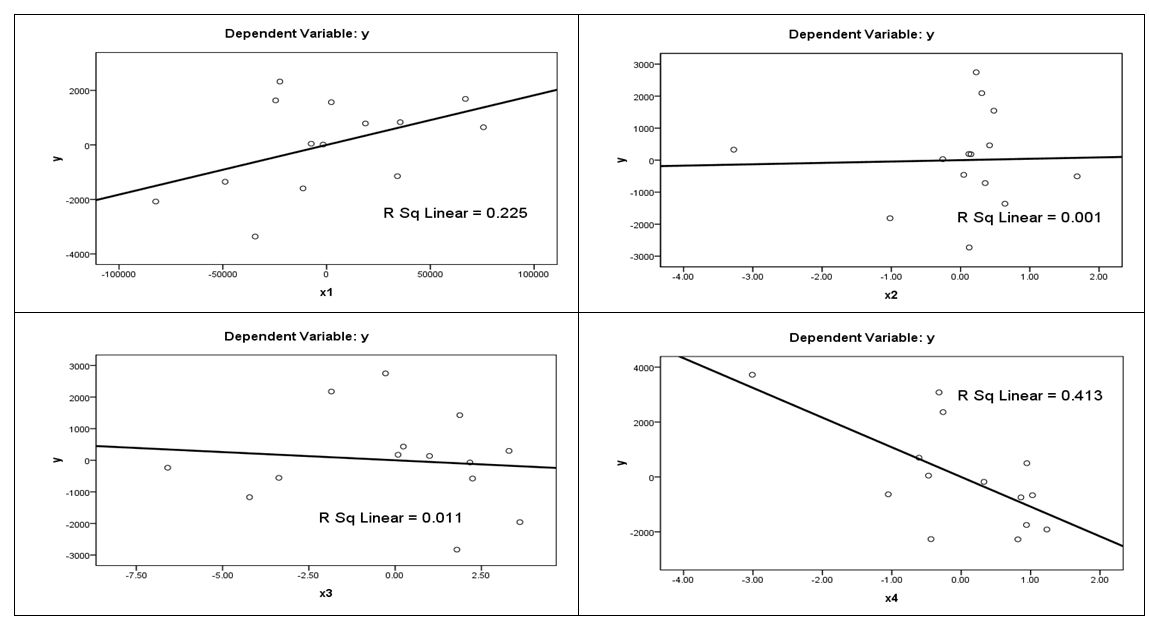
\includegraphics[width=\linewidth]{assets/hospital_partial.png}\end{center}


\par\addvspace{6pt}\noindent\begin{minipage}{\linewidth}

\Question{E17-C6}{高R平方与变量作用排序}

根据表2结果，以下判断哪些正确？

I. 模型决定系数很大，至少有预测应用价值。

\begin{enumerate}
\def\labelenumi{\Roman{enumi}.}
\setcounter{enumi}{1}
\item
  各自变量作用大小依次为X1\textgreater X2\textgreater X3\textgreater X4。
\item
  各自变量作用大小依次为X4\textgreater X1\textgreater X2\textgreater X3。
\end{enumerate}


\begin{choices}

\item 仅I

\item 仅II

\item 仅III

\item I \& III

\item I、II、III均不正确

\end{choices}

\end{minipage}\par\vspace{4pt}

\par\addvspace{6pt}\noindent\begin{minipage}{\linewidth}

\Question{E17-C7}{删去一个变量后的系数}

若Y对X1、X2、X3建模,估计偏回归系数从大到小(不考虑绝对值)排列为


\begin{choices}

\item X1 X3 X2

\item X2 X1 X3

\item X3 X2 X1

\item X1 X2 X3

\item X2 X3 X1

\end{choices}

\end{minipage}\par\vspace{4pt}

\par\addvspace{6pt}\noindent\begin{minipage}{\linewidth}

\Question{E17-C8}{识别强影响观测}

模型的强影响点是OBS


\begin{choices}

\item 4\&11

\item 5

\item 7\&14

\item 14

\item 无强影响点

\end{choices}

\end{minipage}\par\vspace{4pt}

\par\addvspace{6pt}\noindent\begin{minipage}{\linewidth}

\Question{E17-C9}{变量相关不等于误差不独立}

以下哪些说法正确？

I. 根据专业知识，X2和X3不符合LINE中的I条件。

\begin{enumerate}
\def\labelenumi{\Roman{enumi}.}
\setcounter{enumi}{1}
\item
  需要结合偏相关分析判断Y是否独立。
\item
  根据已有统计信息，可断定Y存在序列相关。
\end{enumerate}


\begin{choices}

\item 仅I

\item 仅II

\item 仅III

\item I \& III

\item I、II、III均不正确

\end{choices}

\end{minipage}\par\vspace{4pt}

\par\addvspace{6pt}\noindent\begin{minipage}{\linewidth}

\Question{E17-C10}{住院模型的改进}

本例分析改进的建议,合理的是 I: 将X2剔除\\
II:使用岭回归\\
III:考虑某种时间序列模型


\begin{choices}

\item 仅I

\item 仅II

\item 仅III

\item II \& III

\item I \& II \&III

\end{choices}

\end{minipage}\par\vspace{4pt}

\par\addvspace{6pt}\noindent\begin{minipage}{\linewidth}

\Question{E17-L2}{剔除春节数据后的变化}

如果作者推测春节对急诊量的影响是正确的,则剔除春节期间数据建模,则可能出现的情况是 I. 模型的决定系数变大 II. 偏回归系数的P值变大 III. 偏回归系数绝对值变大


\begin{choices}

\item 仅I

\item 仅II

\item 仅III。

\item I II

\item I III

\item 不能仅据题设确定这些指标的变化方向。

\end{choices}

\end{minipage}\par\vspace{4pt}

\par\addvspace{6pt}\noindent\begin{minipage}{\linewidth}

\Question{E17-L3}{每日资料的独立性风险}

你认为本文存在的致命缺陷是


\begin{choices}

\item 共线性问题导致参数估计结果难以理解

\item 违反线性假设导致模型不``正确''

\item 违反正态性或等方差假设导致参数估计和置信区间不准确

\item 违反独立性假设导致增大I型错误

\item 未给出拟合优度统计量评估模型的应用价值

\end{choices}

\end{minipage}\par\vspace{4pt}

\par\addvspace{6pt}\noindent\begin{minipage}{\linewidth}

\Question{E17-L4}{旧文献的统计表述}

本文论述不妥或错误之处不含


\begin{choices}

\item 关于回代符合率与R2的论述

\item 样本回归方程的书写格式

\item 使用冠心病发病概率的回归模型为线性回归的范例

\item 表1关于假变量(标识变量)的定义

\item 关于共线性的的论述

\end{choices}

\end{minipage}\par\vspace{4pt}

\par\addvspace{6pt}\noindent\begin{minipage}{\linewidth}

\Question{E17-L10}{两年率资料的模型前提}

本文的多重线性回归分析存在的最大问题是


\begin{choices}

\item 婴儿死亡率不服从正态分布

\item 共线性问题

\item 未报告拟合优度统计量

\item 可能不满足独立性假设

\item 未考察线性假设

\end{choices}

\end{minipage}\par\vspace{4pt}

\par\addvspace{6pt}\noindent\begin{minipage}{\linewidth}

\Question{E21-2}{三种残差的分布}

多重线性回归模型,如果满足LINE条件,则 I、标准化残差服从标准正态分布 II、学生化残差服从t分布 III、粗残差估计值均值为0,标准差为剩余标准差


\begin{choices}

\item I

\item II

\item III

\item I\&II\&III

\item 全错

\end{choices}

\end{minipage}\par\vspace{4pt}

\par\addvspace{6pt}\noindent\begin{minipage}{\linewidth}

\Question{E21-4}{正态性是条件假设}

关于回归分析的正态和等方差条件,错误的是


\begin{choices}

\item 给定X条件下Y为正态分布。

\item 可以用Y的边际经验分布与正态分布的吻合判断回归的正态性假设。

\item 可以用粗残差的PP或QQ图初步判断正态性。

\item 可用残差对Y拟合值的散点图判断等方差性。

\item 在模型假设下，不同X取值处的Y条件方差相等。

\end{choices}

\end{minipage}\par\vspace{4pt}

\par\addvspace{6pt}\noindent\begin{minipage}{\linewidth}

\Question{E21-5}{影响点敏感性分析}

多重线性回归统计分析时,发现存在强影响点,则适宜的处理方法是


\begin{choices}

\item 同时报告基于原始数据的模型和删去强影响点的模型

\item 报告更符合自己专业预期的模型

\item 报告基于原始数据的模型

\item 报告删去强影响点的模型

\item 重新收集数据以避免强影响点的影响

\end{choices}

\end{minipage}\par\vspace{4pt}

\par\addvspace{6pt}\noindent\begin{minipage}{\linewidth}

\Question{E21-19}{Durbin–Watson的直接计算}

如果某模型残差依照时间顺序为(0.2, 0.03, 0.4, 0.5, -0.1, 0.02, -0.7, -0.1),则其Durbin-Watson统计量是(拍照没拍全,数据可能不对)


\begin{choices}

\item 0.80

\item 0.89

\item 0.92

\item 0.96

\item 1.11

\item 1.486（按题中所记残差计算）。

\end{choices}

\end{minipage}\par\vspace{4pt}

\par\addvspace{6pt}\noindent\begin{minipage}{\linewidth}

\Question{E21-9}{杠杆与影响度}

关于高杠杆点和强影响点，哪项正确？


\begin{choices}

\item 高杠杆点必有最大粗残差。

\item 高杠杆表示X空间位置特殊，但是否强影响还取决于残差等信息。

\item Cook距离只反映结局绝对大小。

\item 一见高杠杆就必须删除。

\item 杠杆值与自变量无关。

\end{choices}

\end{minipage}\par\vspace{4pt}

\par\addvspace{6pt}\noindent\begin{minipage}{\linewidth}

\Question{N19-8}{VIF与容忍度}

若 \(X_j\) 对其余解释变量回归的 \(R_j^2=.95\)，则VIF为：


\begin{choices}

\item 0.05。

\item 0.95。

\item 1.05。

\item 20。

\item 95。

\end{choices}

\end{minipage}\par\vspace{4pt}

\par\addvspace{6pt}\noindent\begin{minipage}{\linewidth}

\Question{N19-9}{DW的无相关参考值}

残差一阶自相关很弱时，DW通常接近：


\begin{choices}

\item 0。

\item 1。

\item 2。

\item 3。

\item 4。

\end{choices}

\end{minipage}\par\vspace{4pt}

\par\addvspace{6pt}\noindent\begin{minipage}{\linewidth}

\Question{N19-10}{Cook距离的含义}

Cook距离主要衡量：


\begin{choices}

\item 删除单个观测对整体拟合或系数的影响。

\item 某观测的Y值有多大。

\item 某自变量的样本均值。

\item 结局是否正态的P值。

\item 两组样本量差异。

\end{choices}

\end{minipage}\par\vspace{4pt}

\par\addvspace{6pt}\noindent\begin{minipage}{\linewidth}

\Question{N19-11}{正态性检查对象}

回归的经典正态假设主要针对：


\begin{choices}

\item 给定设计后的误差。

\item X的边际分布。

\item Y的边际分布必为单峰正态。

\item X与Y联合必相互独立。

\item 回归系数原始数值。

\end{choices}

\end{minipage}\par\vspace{4pt}

\par\addvspace{6pt}\noindent\begin{minipage}{\linewidth}

\Question{N19-12}{异方差稳健标准误}

采用异方差稳健标准误后，哪项最准确？


\begin{choices}

\item 不改变OLS点估计，仅改变适当条件下的方差估计与推断。

\item 自动修正了遗漏的非线性。

\item 自动消除所有混杂。

\item 使残差必然正态。

\item 让新个体预测永远准确。

\end{choices}

\end{minipage}\par\vspace{4pt}

\par\addvspace{6pt}\noindent\begin{minipage}{\linewidth}

\Question{N19-13}{模型选择与验证泄漏}

在交叉验证中筛选变量、选变换和岭参数，应如何处理？


\begin{choices}

\item 仅在各训练折内完成，再评估验证折。

\item 先用全数据选好，再声称验证完全独立。

\item 只看训练误差最小。

\item 根据验证折结局修改原始数据。

\item 忽略分组或时间结构随机打散所有观测。

\end{choices}

\end{minipage}\par\vspace{4pt}

\par\addvspace{6pt}\noindent\begin{minipage}{\linewidth}

\Question{N19-21}{急诊文章的日均数核查}

按急诊共用资料，199649人次除以730天，平均每日约为：


\begin{choices}

\item 273.49。

\item 274.50。

\item 199.65。

\item 730.00。

\item 285.48。

\end{choices}

\end{minipage}\par\vspace{4pt}

\par\addvspace{6pt}\noindent\begin{minipage}{\linewidth}

\Question{N19-22}{回归系数与标准误}

急诊文中平均相对湿度B=1.011、SE=.159，则检验该系数为0的t值约为：


\begin{choices}

\item 0.157。

\item 0.244。

\item 6.36。

\item 1.011。

\item 无法由这两个数计算。

\end{choices}

\end{minipage}\par\vspace{4pt}

\Needspace{7\baselineskip}\subsubsection*{共用资料：生命质量文章的回归结果}

同文以生命质量总分为结局，报告如下最终多元回归。焦虑/抑郁用原始得分，病程用月，癫痫0否1是，病理分级与文化程度分别按1---4有序编码。

\begin{center}\small\setlength{\tabcolsep}{3.5pt}\renewcommand{\arraystretch}{1.18}\begin{tabular}{@{}lrrrrr@{}}
\toprule
变量 & B & SE & 标准化\(\beta\) & t & P \\
\midrule

截距 & 74.033 & 1.543 & --- & 47.974 & \textless.01 \\
焦虑 & -0.884 & 0.204 & -0.385 & -4.326 & \textless.01 \\
抑郁 & -0.655 & 0.225 & -0.263 & -2.906 & \textless.01 \\
病程 & 0.056 & 0.022 & 0.158 & 2.518 & \textless.05 \\
癫痫 & -4.902 & 1.301 & -0.233 & -3.768 & \textless.01 \\
病理分级 & -0.987 & 0.412 & -0.156 & -2.396 & \textless.05 \\
文化程度 & 0.905 & 0.393 & 0.148 & 2.302 & \textless.05 \\
\bottomrule\end{tabular}\end{center}

文中报告 \(F=22.554\)、\(R^2=.539\)、调整 \(R^2=.517\)。


\par\addvspace{6pt}\noindent\begin{minipage}{\linewidth}

\Question{N19-26}{R平方与调整R平方}

生命质量模型报告R²=.539、调整R²=.517。关于训练样本平方和比例，正确的是：


\begin{choices}

\item 普通R²表示相对于仅截距模型解释了53.9\%的总平方和。

\item 普通R²等于51.7\%。

\item 调整R²保证模型无偏。

\item 该模型已证明外部预测同样好。

\item 余下全部变异均为测量错误。

\end{choices}

\end{minipage}\par\vspace{4pt}

\subsection{简答题}

\par\addvspace{6pt}\noindent\begin{minipage}{\linewidth}

\Question{S20-2}{异方差残差图}

方差不等的典型残差图呈何种形态？手绘示意并简要说明（原题要求提交手绘照片）。


\worklines{3}

\end{minipage}\par\vspace{4pt}

\subsection{计算与分析题}

\Needspace{7\baselineskip}\subsubsection*{共用资料：数学、语文与智商数据}

以智商为y，数学为x1，语文为x2。原卷data1未独立附上，本包补入同课程``语文数学智商.sav''（18人）作数值复算；若原卷数据有改动，需重新代入。


\par\addvspace{6pt}\noindent\begin{minipage}{\linewidth}

\Question{C20-1b}{智商模型的共线性与岭回归}

继续分析智商数据： 1. 计算指标作共线性诊断。 2. 做岭回归、绘制岭迹图，选择岭参数并说明依据。 3. 给出岭参数k=0.12时的原尺度回归方程。


\worklines{3}

\end{minipage}\par\vspace{4pt}

\Needspace{7\baselineskip}\subsubsection*{共用资料：父母与子女身高数据}

y为子女身高，x1为父亲身高，x2为母亲身高。正文同名数据与附带2023 data1逐值一致；以下保留原数据单位，不擅自转换为厘米。

\begin{center}\small\setlength{\tabcolsep}{3.5pt}\renewcommand{\arraystretch}{1.18}\begin{tabular}{@{}lrrr@{}}
\toprule
观测 & 父x1 & 母x2 & 子y \\
\midrule

1 & 5.2 & 4.9 & 6.2 \\
2 & 5.4 & 5.1 & 5.9 \\
3 & 6.2 & 5.5 & 6.6 \\
4 & 5.8 & 5.4 & 6 \\
5 & 5.6 & 5.1 & 6.2 \\
6 & 5 & 4.9 & 5.6 \\
7 & 6.4 & 5.6 & 6.6 \\
8 & 6 & 5.4 & 6.5 \\
\bottomrule\end{tabular}\end{center}


\par\addvspace{6pt}\noindent\begin{minipage}{\linewidth}

\Question{C21-1b}{身高模型的岭迹与k=0.11}

对身高数据： 1. 计算共线性指标。 2. 绘制岭迹图，选岭参数并说明理由。 3. 给出k=0.11时的岭回归方程。


\worklines{3}

\end{minipage}\par\vspace{4pt}

\par\addvspace{6pt}\noindent\begin{minipage}{\linewidth}

\Question{C19-1}{父母身高的岭回归复习题}

对父母子身高数据进行共线性分析，再作岭回归、选择岭参数并写出回归模型。


\worklines{3}

\end{minipage}\par\vspace{4pt}

\par\addvspace{6pt}\noindent\begin{minipage}{\linewidth}

\Question{C19-2}{非线性关系与LINE诊断}

原题给一个SPSS文件，含4个自变量和1个因变量，要求拟合多重线性回归并诊断LINE。回忆提示某个自变量与结局明显呈反比例关系，需用1/x替换后重新拟合。

原4自变量文件未附；这里改用正文中的``线性假设诊断''数据（3个解释变量），只作方法演示。


\worklines{3}

\end{minipage}\par\vspace{4pt}

\Needspace{7\baselineskip}\subsubsection*{共用资料：1990—2003年住院人次及模型诊断}

\begin{center}\small\setlength{\tabcolsep}{3.5pt}\renewcommand{\arraystretch}{1.18}\begin{tabular}{@{}lrrrrr@{}}
\toprule
年份 & 住院人次Y & 门诊X1 & 周转率X2 & 使用率X3 & 住院日X4 \\
\midrule

1990 & 11501 & 454220 & 14.42 & 93.38 & 24.14 \\
1991 & 11512 & 496556 & 14.43 & 90.81 & 23.73 \\
1992 & 11504 & 480663 & 14.36 & 90.31 & 23.73 \\
1993 & 11841 & 445274 & 14.11 & 88.75 & 22.64 \\
1994 & 12096 & 427614 & 9.1 & 82.84 & 22.46 \\
1995 & 11648 & 461228 & 13.92 & 82.53 & 21.93 \\
1996 & 11622 & 391975 & 13.84 & 81.15 & 21.6 \\
1997 & 14892 & 439554 & 17.81 & 92.05 & 19.12 \\
1998 & 18928 & 533686 & 22.82 & 91.86 & 15.08 \\
1999 & 21651 & 605660 & 23.13 & 91.84 & 14.68 \\
2000 & 24673 & 597541 & 24.74 & 91.61 & 13.5 \\
2001 & 28305 & 592311 & 25.1 & 88.63 & 12.7 \\
2002 & 27864 & 590564 & 24.6 & 85.98 & 12.58 \\
2003 & 28691 & 756273 & 27.2 & 84.56 & 12.18 \\
\bottomrule\end{tabular}\end{center}

X2为年出院人数/床位数；X3为占用总床日数/开放总床日数；X4为平均住院日。原表2：

\begin{center}\small\setlength{\tabcolsep}{3.5pt}\renewcommand{\arraystretch}{1.18}\begin{tabular}{@{}lrrrrr@{}}
\toprule
变量 & B & SE & 标准化\(\beta\) & t & P \\
\midrule

截距 & 33058.528 & 12905.767 & --- & 2.562 & 0.031 \\
X1 & 0.0176 & 0.011 & 0.243 & 1.569 & 0.151 \\
X2 & 45.151 & 445.16 & 0.034 & 0.095 & 0.927 \\
X3 & -56.103 & 162.181 & -0.032 & -0.346 & 0.737 \\
X4 & -1100.129 & 436.507 & -0.736 & -0.52 & 0.033 \\
\bottomrule\end{tabular}\end{center}

原表报告 \(R^2=.958\)，调整 \(R^2=.939\)。以下诊断也按原卷保留。

\begin{center}\small\setlength{\tabcolsep}{3.5pt}\renewcommand{\arraystretch}{1.18}\begin{tabular}{@{}lrrrr@{}}
\toprule
观测 & 残差 & 残差标准误 & Student残差 & Cook D \\
\midrule

1 & 1525 & 1449 & 1.052 & 0.109 \\
2 & 186.8319 & 1492.8 & 0.125 & 0.001 \\
3 & 445.4631 & 1536.9 & 0.29 & 0.006 \\
4 & 178.2094 & 1651.5 & 0.108 & 0 \\
5 & 468.4283 & 446.7 & 1.049 & 3.238 \\
6 & -1388 & 1503.1 & -0.924 & 0.066 \\
7 & -577.5792 & 1093.9 & -0.528 & 0.09 \\
8 & -460.7536 & 1498.2 & -0.308 & 0.008 \\
9 & -2734 & 1555.1 & -1.758 & 0.184 \\
10 & -1770 & 1539.1 & -1.15 & 0.086 \\
11 & 43.0857 & 1576.1 & 0.0273 & 0 \\
12 & 2735 & 1575.9 & 1.735 & 0.158 \\
13 & 2080 & 1537.1 & 1.353 & 0.12 \\
14 & -730.8267 & 892.2 & -0.819 & 0.395 \\
\bottomrule\end{tabular}\end{center}

\begin{center}\small\setlength{\tabcolsep}{3.5pt}\renewcommand{\arraystretch}{1.18}\begin{tabular}{@{}lr@{}}
\toprule
变量 & VIF \\
\midrule

X1 & 5.13579 \\
X2 & 27.61614 \\
X3 & 1.87395 \\
X4 & 17.71312 \\
\bottomrule\end{tabular}\end{center}

\begin{center}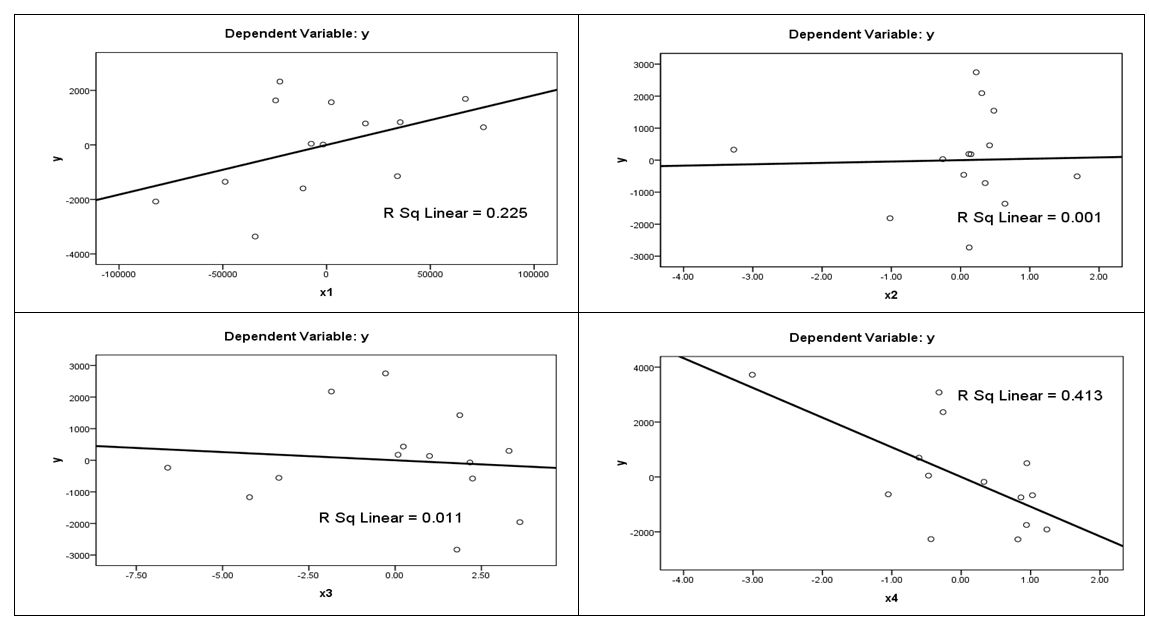
\includegraphics[width=\linewidth]{assets/hospital_partial.png}\end{center}


\par\addvspace{6pt}\noindent\begin{minipage}{\linewidth}

\Question{C20-2}{住院人次：逐步回归与诊断}

以y为住院人次，x1---x4的定义见共用资料，对data2作逐步回归。 1. 写出最终回归方程和拟合优度。 2. 计算指标考察独立性。 3. 列出最大的中心化杠杆、学生化残差、Cook距离及对应观测（原稿此句末尾缺失，本书按年份及数值补齐）。


\worklines{3}

\end{minipage}\par\vspace{4pt}

\par\addvspace{6pt}\noindent\begin{minipage}{\linewidth}

\Question{C21-2}{住院人次：偏回归图与时间顺序}

对同定义的住院data2资料作逐步回归。 1. 写出回归方程和拟合优度。 2. 绘图作线性诊断。 3. 计算指标考察独立性。 4. 列出最大的中心化杠杆、学生化残差、Cook距离，给出年份与数值。


\worklines{3}

\end{minipage}\par\vspace{4pt}



\clearpage\section{补充练习}

本节为配合正文新编的补充练习，按题型排列，题号接续本章往年题，解析见章末。

\subsection{单项选择题}

\par\addvspace{6pt}\noindent\begin{minipage}{\linewidth}

\Question{X26-2-1}{DW检验的不确定区间}

对有时间顺序的资料作回归，得到 \(DW=1.30\)。按题设检验水平、样本量及自变量数查表得 \(d_L=1.10\)、\(d_U=1.50\)。根据正文给出的DW区间判定法，最恰当的结论是：


\begin{choices}

\item 已证实存在一阶正自相关。

\item 已证实存在一阶负自相关。

\item 已证实不存在一阶自相关。

\item DW小于2，因此必定违反所有LINE条件。

\item 对一阶正自相关的判定不确定，需进一步考察。

\end{choices}

\end{minipage}\par\vspace{4pt}

\par\addvspace{6pt}\noindent\begin{minipage}{\linewidth}

\Question{X26-2-2}{条件指数与VIF的联合判断}

三个解释变量的相关阵特征值为2.500、0.499、0.001，其中 \(X_1\) 对其余两个解释变量回归的 \(R_1^2=0.96\)。以下说法正确的是：


\begin{choices}

\item 最大条件指数为2500，\(VIF_1=0.04\)。

\item 最大条件指数为50，说明相关阵必不可逆。

\item 最大条件指数为50，\(VIF_1=25\)，提示严重但非完全共线性。

\item 容忍度为25，说明共线性很弱。

\item 只要3个特征值之和为3，就不存在共线性。

\end{choices}

\end{minipage}\par\vspace{4pt}

\par\addvspace{6pt}\noindent\begin{minipage}{\linewidth}

\Question{X26-2-3}{按相关阵计算岭系数}

两个解释变量与结局均已标准化，给定 \[R_{XX}=\begin{pmatrix}1&0.9\\0.9&1\end{pmatrix},\qquad
r_{XY}=\begin{pmatrix}0.8\\0.7\end{pmatrix}.\] 按正文定义 \(b^*(k)=(R_{XX}+kI)^{-1}r_{XY}\)，取 \(k=0.10\)。两个标准化岭系数依次为：


\begin{choices}

\item \((0.8947,-0.1053)\)。

\item \((0.6250,0.1250)\)。

\item \((0.8000,0.7000)\)。

\item \((0.1250,0.6250)\)。

\item \((0.7273,0.6364)\)。

\end{choices}

\end{minipage}\par\vspace{4pt}

\subsection{简答题}

\Question{X26-2-4}{偏回归图的代码纠错}

要考察控制 \(X_2,X_4\) 后 \(X_3\) 与Y的线性关系，某同学写出：

\begin{verbatim}
u <- resid(lm(x3 ~ x2 + x4, data = d))
v <- resid(lm(y ~ x2 + x3 + x4, data = d))
plot(u, v)
\end{verbatim}

假设资料无缺失、模型满列秩。指出代码中的关键问题，写出正确代码，并说明为什么原图可能让人误判为``X3与Y无关''。


\worklines{3}

\subsection{计算与分析题}

\Question{X26-2-5}{小样本的离群与杠杆诊断}

对下列数据拟合含截距的一元线性回归：

\begin{center}\small\setlength{\tabcolsep}{5pt}\renewcommand{\arraystretch}{1.18}\begin{tabular}{@{}llllll@{}}
\toprule
观测号 & 1 & 2 & 3 & 4 & 5 \\
\midrule

X & 1 & 2 & 3 & 4 & 5 \\
Y & 3.4 & 7.9 & 14.6 & 13.6 & 15.5 \\
\bottomrule\end{tabular}\end{center}

本题按正文经验标准筛查：\(|r_{i(\text{外})}|>3\) 提示Y方向离群；\(h_{ii}>2\bar h\) 提示高杠杆；Cook \(D_i>1\) 提示强影响。

\begin{enumerate}
\def\labelenumi{\arabic{enumi}.}
\tightlist
\item
  给出回归方程、剩余标准差及第3号观测的粗残差、杠杆值、内学生化残差、外学生化残差、Cook距离；据此判断第3号观测。
\item
  加入第6号观测 \((X_6,Y_6)=(10,33)\) 后重新拟合，计算第6号观测的杠杆值、外学生化残差、Cook距离，并判断其属于哪类可疑观测。
\item
  说明两问的结果为何不矛盾，以及发现可疑观测后的处理原则。
\end{enumerate}


\worklines{3}

\clearpage\section{习题解析}

\begin{keyidea}[核对方式]题号与前文一一对应。补写范围、原题歧义及数据还原方法列在相应答案中。\end{keyidea}

\Answer{E14-14}{拟合优度与应用价值}

\textbf{答案：E。}

R²是否有用取决于领域、目标和验证表现，没有通用0.8或0.9门槛。加入变量会使训练R²不降，不能单靠最大化它筛选；调整R²也不是无条件无偏或预测可靠性的证明。


\Answer{E14-15}{回归的前提条件}

\textbf{答案：C。}

回归并不要求结局与自变量相互独立，否则通常也无关系可建模。独立性主要指给定设计后观测误差相互独立；正态性用于经典小样本推断，正态假定针对条件误差而不是边际Y。


\Answer{E14-16}{文献报告不足与已证实错误}

\textbf{答案：E较符合``不包括''的意图。}

未展示散点图不能证明作者没有检查过线性，且线性应结合专业关系、函数形式和残差/偏残差考察。文章确实未报告本模型拟合优度；表中SE中文写成``标准物''是笔误。时间相关及共线性是应检查的风险，不能在无原始数据时声称已由检验证实。


\Answer{E14-17}{讨论与模型是否一致}

\textbf{答案：D。}

讨论提到高温和低温都可能增加急症，而拟合式以最高、最低气温的正线性项描述关系，并未给出U形等非线性证据。应区分研究自身模型结果与引用或推测，避免把讨论中的机制解释当成已验证结果。


\Answer{E14-19}{原文统计表述辨析}

\textbf{答案：待原文核实。}

选项涉及文章对拟合优度、模型前提、哑变量和系数的具体陈述；原文未附，无法可靠指定错误项。可核对条件分布而非边际正态、参照编码以及概率与优势的区别。


\Answer{E14-20}{率的变换与分析}

\textbf{答案：C是通常可接受的方法选项，仍需原文核实。}

对比例作平方根反正弦变换是传统可用方法之一，本身不能直接定为错误；是否适合还取决于分母、边界与方差结构。两年同一单位的率可能相关，且统计关联不能证明降低出生率会降低婴儿死亡率。


\Answer{E14-21}{将伴随关系解释为因果}

\textbf{答案：D。}

若仅凭观察性回归即说降低出生率能够降低婴儿死亡率，属于把关联上升为因果干预效果。原文未附，能够评价的是选项所描述的推论，不能断言文章其他部分是否还有更大问题。


\Answer{E17-M3}{LINE中的独立性}

\textbf{答案：B。}

指不同观察单位的误差在给定自变量后独立；不是Y与X独立，也不是各自变量必须独立。B是原选项最接近的表述。


\Answer{E17-M5}{独立性如何判断}

\textbf{答案：B（一般情形）。}

独立性首先取决于抽样和研究设计。对有时间顺序的数据，DW和残差时序图是辅助诊断，因此A、D在相应场景也有用；任何单一图或检验都不能证明任意依赖形式不存在。


\Answer{E17-M9}{R平方的使用}

\textbf{答案：E。}

小R²也可能有研究或预测价值，但仍须评估误差、校准及验证。统计显著不自动等于重要，调整R²也不保证无偏。


\Answer{E17-M13}{预测价值的证据}

\textbf{答案：C。}

独立外部样本上的预测误差最有说服力。训练残差、R²或学生化残差都不能替代对新数据的预测评估；数据预处理与选择也不能泄漏外部样本信息。


\Answer{E17-M14}{强影响点的处理}

\textbf{答案：A。}

先核对录入、测量和样本是否符合纳入规则；无确证错误时不随意删除。报告包含与不包含该点的敏感性分析，说明系数、结论如何变化，避免按预期结果选模型。


\Answer{E17-M15}{等方差的图形诊断}

\textbf{答案：E。}

看残差相对拟合值或自变量的散点，漏斗形等模式提示方差随均值改变。


\Answer{E17-M17}{控制智商后的成绩关系}

\textbf{答案：C。}

分别剔除智商等协变量的线性作用后，可用偏回归/残差散点考察两科成绩的条件关系。


\Answer{E17-M18}{正态性的图形诊断}

\textbf{答案：D。}

应看模型残差的QQ图，重点是条件误差分布；不能只看原始Y的边际分布。


\Answer{E17-C6}{高R平方与变量作用排序}

\textbf{答案：E。}

高训练R²本身不证明预测价值。变量量纲不同，且X2/X4共线性严重、有强影响点，不能据单次全模型系数直接确定稳健贡献排序；III即便符合表中标准化绝对值排序，也不等于可靠的因果或预测贡献。


\Answer{E17-C7}{删去一个变量后的系数}

\textbf{答案：B。}

对原表1转录资料拟合 \(Y\sim X_1+X_2+X_3\)，得到系数约0.01054、1057.35、−311.08，因此按代数值降序为 \(X_2>X_1>X_3\)。不要按旧模型系数直接删除一项而不重新拟合。


\Answer{E17-C8}{识别强影响观测}

\textbf{答案：B。}

原输出第5个观测Cook D约3.238，明显突出；该点对应1994年。其学生化残差未必很大，因为高杠杆点可将回归面拉向自身。


\Answer{E17-C9}{变量相关不等于误差不独立}

\textbf{答案：E。}

LINE中的I不是要求自变量之间独立。偏相关不能检验时间序列误差独立；原给诊断不足以断定序列相关存在。应结合按时间排列的残差及适当检验。


\Answer{E17-C10}{住院模型的改进}

\textbf{答案：E（作为可研究的候选方案）。}

核对并考虑移除冗余变量、使用岭回归缓解不稳定，以及处理年度时间结构，都是可比较的改进方向。删除X2须有依据并重新拟合；岭回归不自动解决序列相关，时间序列模型也不自动解决错误函数形式。


\Answer{E17-L2}{剔除春节数据后的变化}

\textbf{答案：F（补入：无法仅据题设确定）。}

删除部分日期可能改变暴露分布、残差方差、样本量和系数，因此R²、P值、系数绝对值没有必然方向。需要原数据与明确的节假日效应模型，不能凭叙述决定I/II/III。


\textbf{补写说明。} 原B、C选项均写``仅II''，这里将C补为``仅III''，并加入无法确定变化方向的F项；不宣称F来自原卷。


\Answer{E17-L3}{每日资料的独立性风险}

\textbf{答案：D（优先需要检查的风险）。}

730个连续日期可能存在趋势、季节性或残差自相关；若被忽略，标准误和检验可能不可靠。但论文未给时间残差诊断，不能在没有数据时说已检验证实违反独立性。


\Answer{E17-L4}{旧文献的统计表述}

\textbf{答案：待原文核实。}

选项须对照原文关于线性概率模型、回代符合率、变量赋值和共线性的实际表述；本包未提供该文，不能指定唯一正确项。


\Answer{E17-L10}{两年率资料的模型前提}

\textbf{答案：D是题目提示的主要风险，需原文核验。}

若同一民族或地区提供两个年份的率，它们可能相关，不能简单视为独立观察。原文未附，尚不能确认该研究具体数据结构或其余问题是否更严重。


\Answer{E21-2}{三种残差的分布}

\textbf{答案：B若指外学生化；E若指内部学生化。}

含截距时残差均值为0，但其样本标准差与剩余标准差分别为\[\sqrt{SSE/(n-1)},\qquad s=\sqrt{SSE/(n-p-1)},\]二者不相等，所以III通常错误。以估计的s标准化的残差不严格为标准正态。删点外学生化残差在经典正态模型下有精确t分布；内部学生化不服从该t分布。原稿把II一律判错混淆了定义。


\Answer{E21-4}{正态性是条件假设}

\textbf{答案：B。}

给定X的条件误差正态，不要求混合了不同条件均值的边际Y正态。粗残差QQ图可作初步诊断；杠杆差异大时标准化/学生化更有帮助，但不能说粗残差QQ图本身就是错误。原回忆稿的对错批注不正确。


\Answer{E21-5}{影响点敏感性分析}

\textbf{答案：A。}

先核对录入、测量和样本是否符合纳入规则；无确证错误时不随意删除。报告包含与不包含该点的敏感性分析，说明系数、结论如何变化，避免按预期结果选模型。


\Answer{E21-19}{Durbin–Watson的直接计算}

\textbf{答案：F（补入1.486）。}

按回忆向量，\(DW=\sum_{i=2}^n(e_i-e_{i-1})^2/\sum_{i=1}^n e_i^2=1.4286/0.9613\approx1.48611\)。原A---E均不匹配，说明回忆向量或选项有缺误。保留原向量和选项，补入本向量对应值；R应写 \texttt{sum(diff(e)\^{}2)/sum(e\^{}2)}，避免矩阵乘除优先级错误。


\textbf{补写说明。} 保留回忆残差与原A---E，新增与所记向量一致的F项。原稿注明残差可能没记全。


\Answer{E21-9}{杠杆与影响度}

\textbf{答案：B。}

杠杆来自设计矩阵。强影响常是杠杆与残差共同作用，需检查删除该点后估计如何改变。


\textbf{补写说明。} 原第9题整题未记录，本题新编。


\Answer{N19-8}{VIF与容忍度}

\textbf{答案：D。}

\(VIF=1/(1-R_j^2)=20\)，容忍度0.05。阈值是经验诊断，不应单靠它删去关键变量。


\textbf{补写说明。} 2019回忆稿只给出30道选择的总数及大致范围，没有记录本题原文；本题是依课程内容与所附材料新编的补充练习，不冒作恢复的原试卷。


\Answer{N19-9}{DW的无相关参考值}

\textbf{答案：C。}

近似关系为 \(DW\approx2(1-\hat\rho_1)\)；正式判定仍需对应设计的分布或检验，不能用2作机械界线。


\textbf{补写说明。} 2019回忆稿只给出30道选择的总数及大致范围，没有记录本题原文；本题是依课程内容与所附材料新编的补充练习，不冒作恢复的原试卷。


\Answer{N19-10}{Cook距离的含义}

\textbf{答案：A。}

它结合残差与杠杆信息。可疑观测应核查并作敏感性分析，不宜为得到显著结果而删除。


\textbf{补写说明。} 2019回忆稿只给出30道选择的总数及大致范围，没有记录本题原文；本题是依课程内容与所附材料新编的补充练习，不冒作恢复的原试卷。


\Answer{N19-11}{正态性检查对象}

\textbf{答案：A。}

不同X对应不同条件均值，混合后边际Y可以不呈正态。残差图用于近似诊断，不能把它当独立误差的直接观测。


\textbf{补写说明。} 2019回忆稿只给出30道选择的总数及大致范围，没有记录本题原文；本题是依课程内容与所附材料新编的补充练习，不冒作恢复的原试卷。


\Answer{N19-12}{异方差稳健标准误}

\textbf{答案：A。}

稳健标准误解决的是方差估计问题，不能替代正确均值模型或因果设计。


\textbf{补写说明。} 2019回忆稿只给出30道选择的总数及大致范围，没有记录本题原文；本题是依课程内容与所附材料新编的补充练习，不冒作恢复的原试卷。


\Answer{N19-13}{模型选择与验证泄漏}

\textbf{答案：A。}

所有利用结局的选择都应在训练阶段进行；相关资料还需按个体、组或时间块划分，必要时采用嵌套验证。


\textbf{补写说明。} 2019回忆稿只给出30道选择的总数及大致范围，没有记录本题原文；本题是依课程内容与所附材料新编的补充练习，不冒作恢复的原试卷。


\Answer{N19-21}{急诊文章的日均数核查}

\textbf{答案：A。}

直接相除为273.4918，与文中274.5不一致，应核查总数、天数或报告值。


\textbf{补写说明。} 2019回忆稿只给出30道选择的总数及大致范围，没有记录本题原文；本题是依课程内容与所附材料新编的补充练习，不冒作恢复的原试卷。


\Answer{N19-22}{回归系数与标准误}

\textbf{答案：C。}

\(t=B/SE\approx6.3585\)；但其标称P值是否可靠还取决于误差相关结构等条件。


\textbf{补写说明。} 2019回忆稿只给出30道选择的总数及大致范围，没有记录本题原文；本题是依课程内容与所附材料新编的补充练习，不冒作恢复的原试卷。


\Answer{N19-26}{R平方与调整R平方}

\textbf{答案：A。}

调整R²加入自由度惩罚，不能简单替代原始平方和比例；两者也都不等于样本外表现。


\textbf{补写说明。} 2019回忆稿只给出30道选择的总数及大致范围，没有记录本题原文；本题是依课程内容与所附材料新编的补充练习，不冒作恢复的原试卷。


\Answer{S20-2}{异方差残差图}

常见为漏斗形或喇叭形：残差中心仍大致围绕0，但随拟合值或某自变量变化，竖向散布逐渐增大或减小。

\begin{center}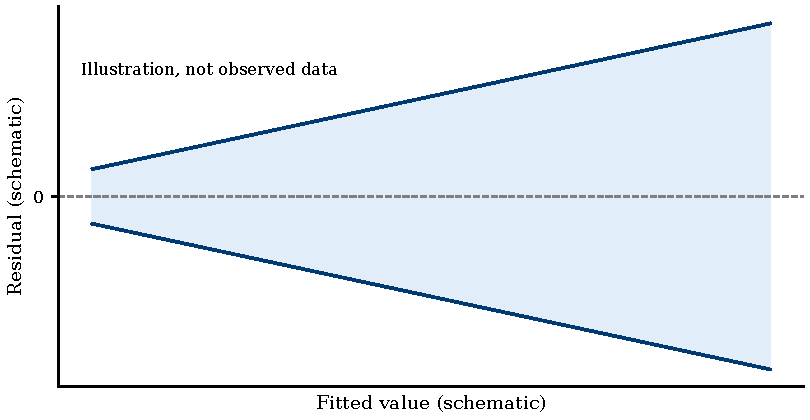
\includegraphics[width=.82\linewidth]{assets/funnel_schematic.pdf}\end{center}

这是数学示意的散布包络，不是实测样本点。还可能出现其他异方差模式，不能只寻找一种形状；需结合变量变换、方差建模或稳健标准误，并先确保均值函数合适。


\Answer{C20-1b}{智商模型的共线性与岭回归}

本书统一采用相关阵尺度的岭参数定义： \[b^*(k)=(R_{XX}+kI)^{-1}r_{XY},\quad b_j(k)=b_j^*(k)\frac{s_Y}{s_{X_j}},\quad b_0(k)=\bar Y-\sum_jb_j(k)\bar X_j.\] 其他软件若以 \(X^TX+\lambda I\) 定义惩罚，参数量级会不同，不能直接混用。

相关系数0.932002；容忍度0.131372；两个变量VIF均为7.611995。以相关阵特征根比平方根定义的条件指数约5.3304。

\begin{center}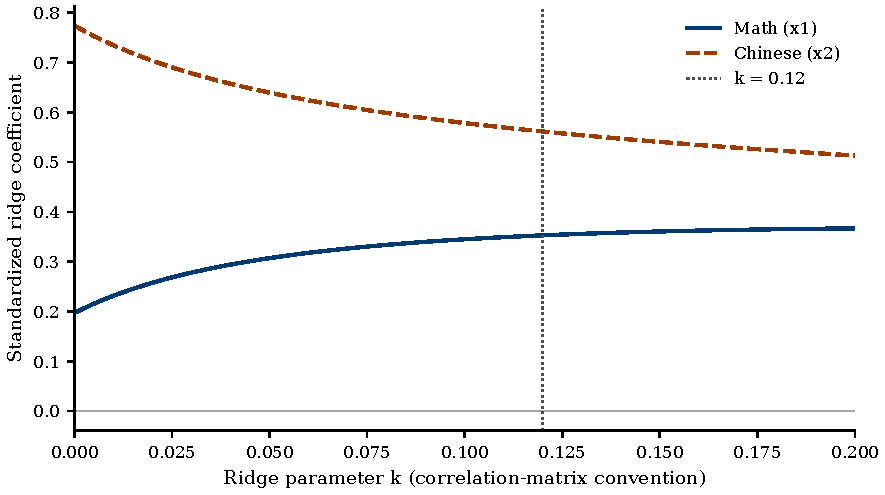
\includegraphics[width=.9\linewidth]{assets/ridge_iq.pdf}\end{center}

k=0.12的原尺度方程为 \[\widehat y=12.092095+0.387816x_1+0.713526x_2.\] 在0---0.20、步长0.005的预设网格中，GCV最小在k=0.04；它与题目指定的0.12不是同一要求。岭迹趋稳可作为辅助，但不应只为让系数``好看''选参数。图中为实算的标准化系数路径，完整网格随代码提供。


\Answer{C21-1b}{身高模型的岭迹与k=0.11}

本书统一采用相关阵尺度的岭参数定义： \[b^*(k)=(R_{XX}+kI)^{-1}r_{XY},\quad b_j(k)=b_j^*(k)\frac{s_Y}{s_{X_j}},\quad b_0(k)=\bar Y-\sum_jb_j(k)\bar X_j.\] 其他软件若以 \(X^TX+\lambda I\) 定义惩罚，参数量级会不同，不能直接混用。

父母身高相关0.974782；容忍度0.049799；VIF均为20.080645；条件指数约8.8493。

\begin{center}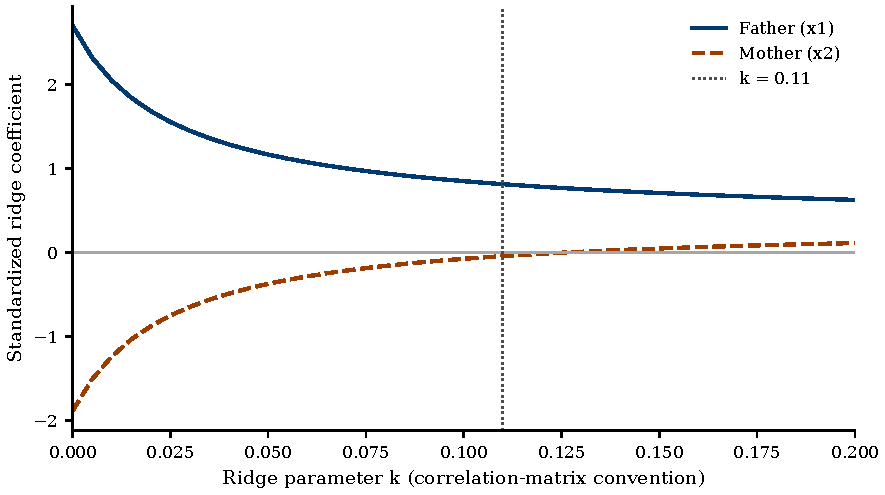
\includegraphics[width=.9\linewidth]{assets/ridge_height.pdf}\end{center}

k=0.11时 \[\widehat y=3.095451+0.595344x_1-0.055162x_2.\] 此时标准化系数为(0.813395,−0.041879)。按每0.01一个k、首列k=0的存储方式，k=0.11应取第12列，不能误取第11列。

\textbf{选参的限制。} 在本包0---0.20、步长0.005网格中，GCV最小在k=0；这与``曲线变稳定''标准不同。因此可以报告正k下的稳定性分析，但不能声称0.11在该数据上已经证明预测最优。


\Answer{C19-1}{父母身高的岭回归复习题}

本书统一采用相关阵尺度的岭参数定义： \[b^*(k)=(R_{XX}+kI)^{-1}r_{XY},\quad b_j(k)=b_j^*(k)\frac{s_Y}{s_{X_j}},\quad b_0(k)=\bar Y-\sum_jb_j(k)\bar X_j.\] 其他软件若以 \(X^TX+\lambda I\) 定义惩罚，参数量级会不同，不能直接混用。

原2019数据未另附，采用正文同名的8条记录演示：VIF约20.0806，说明父母身高的条件系数不稳定。岭迹及原尺度换算可按本章身高题操作。

如指定k=0.11作稳定性展示，方程为 \(\hat y=3.095451+0.595344x_1-0.055162x_2\)；若严格按本包粗网格GCV选择，最小点为k=0，即普通最小二乘。应说明选择标准和小样本局限，而不是把某个正k当作唯一标准答案。


\Answer{C19-2}{非线性关系与LINE诊断}

先检查散点和控制其他变量后的偏残差关系，再检查设计独立性、残差正态与方差结构；同时看异常/强影响点。若专业及图形支持反比例关系，可用 \(1/X_j\) 作为解释项，注意 \(X_j=0\) 的定义和近零值的不稳定性，再重复诊断与验证。

正文3自变量演示数据中，将x1改为倒数使AIC由397.682降至390.610，方程为 \[\hat y=347.5607-606.6008/x_1+4.5034x_2+1.9687x_3.\] 这些数字不冒作2019原卷4自变量的结果；原文件补齐后应按同样步骤分析，不能把case编号作为解释变量凑数。


\Answer{C20-2}{住院人次：逐步回归与诊断}

本包依据原卷表1逐格转录的14年数据，用AIC的双向逐步法，保留x1、x4： \[\widehat y=28825.883+0.0185703x_1-1122.3837x_4.\] \(R^2=0.956916\)，调整 \(R^2=0.949082\)，剩余标准差1613.316。按年份排列残差，\(DW=1.064356\)；\texttt{lmtest::dwtest}双侧P约0.00829，提示该模型的序列相关问题值得处理。

最大中心化杠杆 \(h_i-1/n\) 在2003年，为0.551061；最大绝对外学生化残差在1998年，为−2.30630；代数最大的外学生化残差在2001年，为2.21072；最大Cook D也在2001年，为0.309879。必须说明按绝对值还是代数值选``最大''。

\textbf{版本核对。} 原表2系数与表1转录复算不完全一致，且表中X4的t写作−0.520，与系数/标准误约−2.520不符。旧卷data2没有独立文件，这里明确以可见表1为复算依据；若找到原卷文件，应重新核对。全部逐步选择、残差和年份指标已随代码提供。


\Answer{C21-2}{住院人次：偏回归图与时间顺序}

本包依据原卷表1逐格转录的14年数据，用AIC的双向逐步法，保留x1、x4： \[\widehat y=28825.883+0.0185703x_1-1122.3837x_4.\] \(R^2=0.956916\)，调整 \(R^2=0.949082\)，剩余标准差1613.316。按年份排列残差，\(DW=1.064356\)；\texttt{lmtest::dwtest}双侧P约0.00829，提示该模型的序列相关问题值得处理。

最大中心化杠杆 \(h_i-1/n\) 在2003年，为0.551061；最大绝对外学生化残差在1998年，为−2.30630；代数最大的外学生化残差在2001年，为2.21072；最大Cook D也在2001年，为0.309879。必须说明按绝对值还是代数值选``最大''。

\textbf{版本核对。} 原表2系数与表1转录复算不完全一致，且表中X4的t写作−0.520，与系数/标准误约−2.520不符。旧卷data2没有独立文件，这里明确以可见表1为复算依据；若找到原卷文件，应重新核对。全部逐步选择、残差和年份指标已随代码提供。

最终模型的偏回归图（控制另一个保留变量，14个年份）：

\begin{center}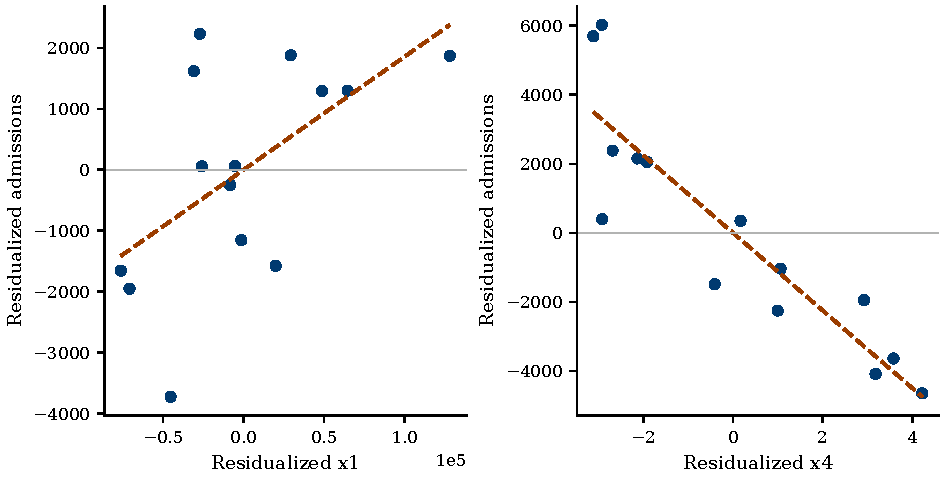
\includegraphics[width=\linewidth]{assets/hospital_partial_recomputed.pdf}\end{center}

直线只作条件关系的图形参照。仅有总体趋势不足以证明线性形式正确；应同时看曲率、影响观测与时间残差，并区分原全模型的偏回归图和这里最终模型的图。

\clearpage\subsection*{补充练习解析}

以下为补充练习的解析。这些题目为配合正文新编，并非往年试题；题中设定的数值仅供练习。

\Answer{X26-2-1}{DW检验的不确定区间}

\textbf{答案：E。}

\(d_L<DW<d_U\)，落在不能确定的区间。\(DW<2\) 可提示正相关方向，但不能替代查表结论，更不能把``不确定''当作``没有自相关''。可继续查看按时间排列的残差图，并采用适合该资料的进一步检验。




\Answer{X26-2-2}{条件指数与VIF的联合判断}

\textbf{答案：C。}

按正文相关阵定义，最大条件指数为 \(\sqrt{2.500/0.001}=50\)；\(VIF_1=1/(1-0.96)=25\)，容忍度0.04。两项均提示严重共线性，但最小特征值仍大于0，不能称为完全共线性。系数可能不稳定，不等于正规方程已无唯一解。




\Answer{X26-2-3}{按相关阵计算岭系数}

\textbf{答案：B。}

\[b^*(0.10)=\frac1{1.1^2-0.9^2}
\begin{pmatrix}1.1&-0.9\\-0.9&1.1\end{pmatrix}
\begin{pmatrix}0.8\\0.7\end{pmatrix}
=\begin{pmatrix}0.625\\0.125\end{pmatrix}.\] 岭惩罚加在计算矩阵的主对角线上，原始变量的样本相关系数仍为0.9。它改变的是估计方法；本题给定的k也不代表已由岭迹选出了最佳参数。




\Answer{X26-2-4}{偏回归图的代码纠错}

第二个辅助回归不应包含待考察的 \(X_3\)；两边都只剔除控制变量 \(X_2,X_4\) 的线性影响。

\begin{verbatim}
u <- resid(lm(x3 ~ x2 + x4, data = d))
v <- resid(lm(y ~ x2 + x4, data = d))
plot(u, v)
abline(lm(v ~ u))
\end{verbatim}

原代码的v是完整回归的残差，与设计矩阵各列正交；u又是这些列的线性组合，故样本内 \(u^Tv=0\)。原图中的线性趋势被构造过程消掉，不能据此说X3没有条件效应。正确图用于考察控制其他变量后的线性关系；图形本身也不是已证明LINE全部成立。




\Answer{X26-2-5}{小样本的离群与杠杆诊断}

\textbf{（1）原5点模型。} \(\hat Y=2.03+2.99X\)，\(s=2.4453\)。第3号观测的结果为：

\begin{center}\small\setlength{\tabcolsep}{5pt}\renewcommand{\arraystretch}{1.18}\begin{tabular}{@{}ll@{}}
\toprule
指标 & 数值 \\
\midrule

粗残差 & 3.6000 \\
杠杆值 & 0.2000 \\
内学生化残差 & 1.6460 \\
外学生化残差 & 4.3164 \\
Cook距离 & 0.3386 \\
\bottomrule\end{tabular}\end{center}

因此第3号按题设标准提示Y方向离群，但其杠杆不高，Cook距离也未超过1。不能仅因内学生化残差未超过3就忽略它。

\textbf{（2）加入第6号后。} 新方程为 \(\hat Y=1.6967+3.1128X\)，\(s=2.1288\)。第6号 \(h_{66}=0.8361\)，\(\bar h=2/6=0.3333\)，故 \(h_{66}>2\bar h\)；其外学生化残差0.1772、Cook距离0.1056。它提示高杠杆，但按题设阈值不提示Y方向离群或强影响。判断须使用6点模型的诊断量。

\textbf{（3）区别与处理。} 外学生化残差以删点后估计的误差方差衡量Y方向偏离；杠杆反映X位置是否特殊；Cook距离综合残差与杠杆。本例第6号虽在X方向较远，却贴近回归线。经验阈值用于筛查，应先核查数据，再比较含该点与不含该点的拟合，不按是否有利于结论选择性删点。

可用R的 \texttt{rstandard()}、\texttt{rstudent()}、\texttt{hatvalues()}、\texttt{cooks.distance()} 复算，完整代码随笔记提供。
\EndExercises
